\documentclass[../thesis]{subfiles}

\begin{document}
	\section{Results}
	\label{sec:mic:results}

	The techniques described in \cref{sec:mic:optims} can not be considered optimizations until their impact in the application performance is properly quantified and evaluated. This section discusses the measurements performed for this purpose, using the same environment and methodology as already described in \cref{subsec:mic:native:results}.

	Performance tests focused mainly on the the techniques described in \cref{subsec:mic:optims:usb,subsec:mic:optims:overwrite} (\usb and OW). Preliminary tests revealed that the first technique (massive parallelism) did not decrease the execution time of the algorithm, and the benefit from the second (loop unrolling) was too little to be significant. Although this was not the case with the third (removed Armadillo) it was used as the base for \usb and OW, since it required a major change to the implementation. When reading the following results, it is important to consider that a significant fraction of the improvements shown by these techniques comes from that.

	Theoretically, the parallelization of the dependency solving step compensates for the lack of parallelism in the more advanced stages of the algorithm. However, tests showed this not to be the case, showing how the memory access pattern hampers further scalability. As the algorithm progresses, the number of dependencies for each element increase, but half of this dependencies lie in distinct cache lines. The lack of locality seems to hamper the algorithm so much that it would nullifies any improvement from increased parallelism.

	% Subsequent research \cite{PRACE:MIC:BestPracticeGuide} revealed the problem to be in the way OpenMP was being used. It was assumed that threads would automatically be spread among nested parallel regions, similar to what happens with the scheduling of threads in a single parallel region, but the truth is that nested parallelism is disabled by default. Consequently, it has to be enabled manually, either through the environment or through a small change in the source code. Additionally, the number of threads for each parallel region also has to be set manually, either through the environment (using comma separated values) or by using the default OpenMP routine to set the number of threads for each region individually. Despite the correction being fairly easy, when the problem was correctly identified there was no time left to rerun the performance tests.

	On the other hand, the lack of performance improvements from loop unrolling did not come as a surprise, serving the purpose of proving how the \intel\xeonphi coprocessor is superior to a \gpu when dealing with conditional branches.

	The execution time for \usb is shown in \cref{fig:mic:optims:usb:times} and, comparing with \cref{fig:mic:block:diagonal:times}, the speedup is clear even for the sequential time (reduced to less than half). The peak performance remained near the same number of threads (30 for $n=2000$, 60 for $n=4000$ and 120 for $n=8000$), but when more threads than those supported by the hardware are demanded, the performance now drops more intensely, with the optimized implementation taking twice as long with 360 threads.

	\begin{figure}[p]
		\centering
		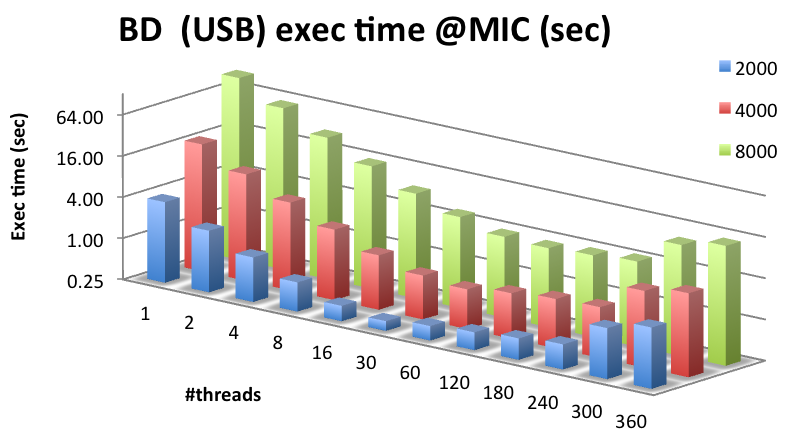
\includegraphics[height=0.25\textheight]{assets/images/mic/optims/mic-usb-times.png}
		% \captionsetup{font=small}
		\caption{Execution times for USB in the \intel\xeonphi coprocessor.}
		\label{fig:mic:optims:usb:times}
	\end{figure}
	
	\begin{figure}[p]
		\centering
		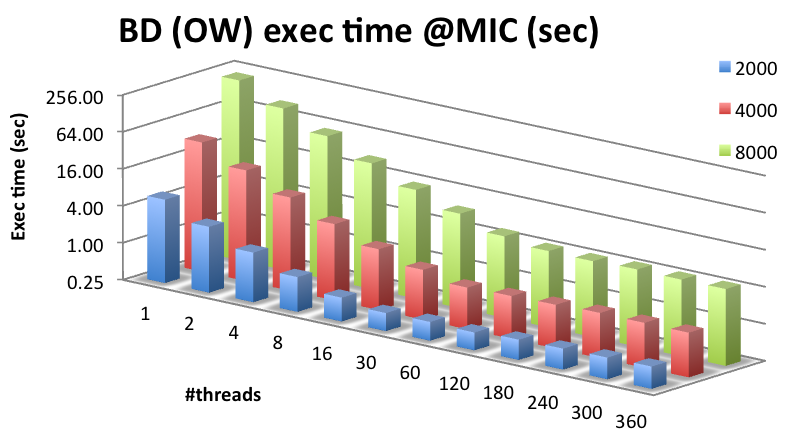
\includegraphics[height=0.25\textheight]{assets/images/mic/optims/mic-ow-times.png}
		% \captionsetup{font=small}
		\caption{Execution times for OW in the \intel\xeonphi coprocessor.}
		\label{fig:mic:optims:ow:times}
	\end{figure}

	\begin{figure}[p]
		\centering
		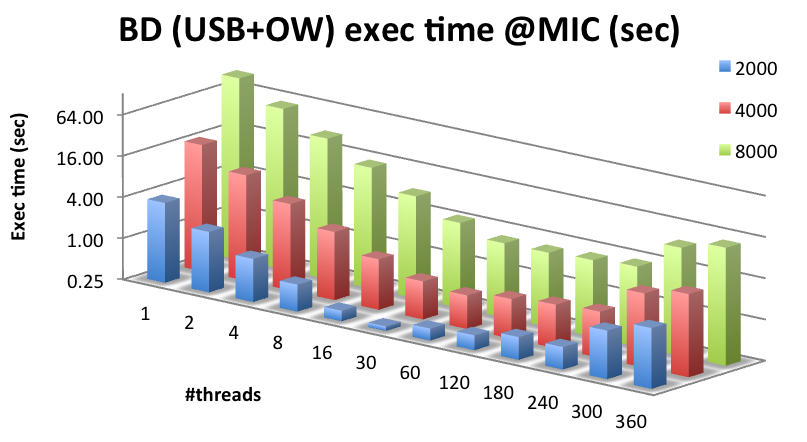
\includegraphics[height=0.25\textheight]{assets/images/mic/optims/mic-usbow-times.png}
		\caption{Execution times for USB and OW in the \intel\xeonphi coprocessor.}
		\label{fig:mic:optims:usbow:times}
	\end{figure}

	While not so good, OW also improves the efficiency of the implementation, as shown in \cref{fig:mic:optims:ow:times}. Contrary to what happens with USB, this optimization practically removes the penalty of demanding more threads than what the hardware supports, maintaining the execution time near peak performance even above 8 threads per core. Yet, the minimum execution time this optimization achieves is not as low.

	Although USB exceeds OW in speedup, the highest efficiency is achieved when using both optimizations at the same time (\cref{fig:mic:optims:usbow:times}). The sequential time and the time obtained with 360 threads are practically the same as for USB only, and the same happens for the peaks. However, the value obtained with these peaks is reduced when OW is also applied.

	\Cref{fig:mic:optims:best:times} shows the best execution times for the naive implementation and each optimization running in the \intel\xeonphi and the best execution time for USB and OW together running on the multicore environment. While it is clear the benefit of both optimizations, there is the problem of these optimizations being common to both the coprocessor and the multicore environment. However, \cref{fig:mic:optims:best:times} shows that these optimizations significantly reduce the speedup gap between the \cpu and the device.

	\begin{figure}[t]
		\begin{minipage}{0.48\textwidth}
			\centering
			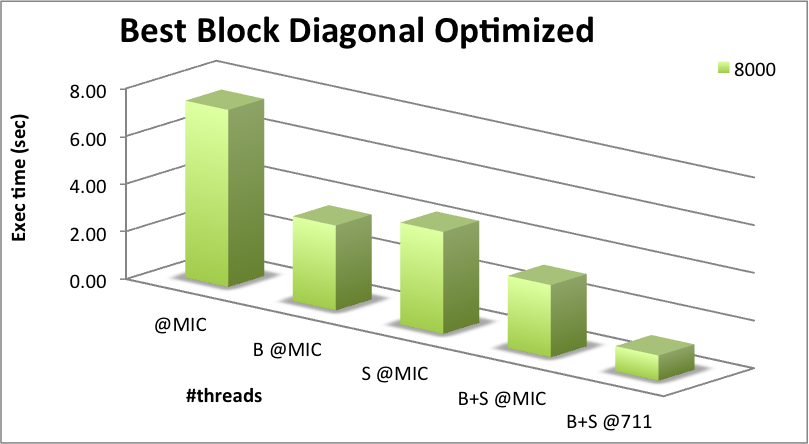
\includegraphics[width=\textwidth]{assets/images/mic/optims/best.png}
			\captionsetup{font=small}
			\caption{Best execution times for the optimizations.}
			\label{fig:mic:optims:best:times}
		\end{minipage}
		\hfill
		\begin{minipage}{0.48\textwidth}
			\centering
			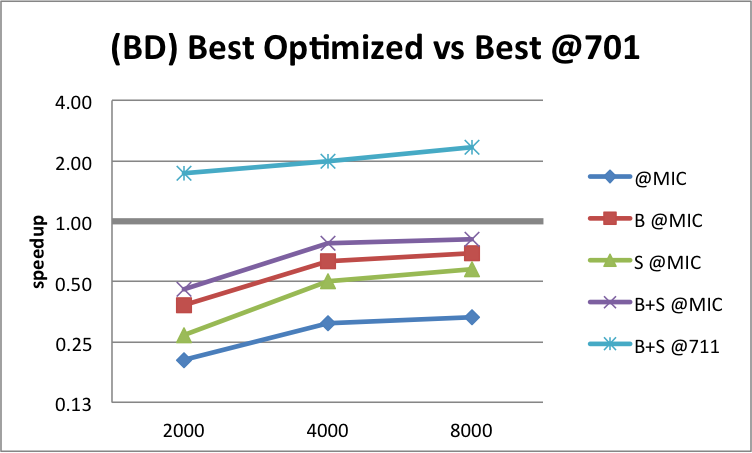
\includegraphics[width=\textwidth]{assets/images/mic/optims/best-speedup.png}
			\captionsetup{font=small}
			\caption{Speedups for the optimizations versus multicore in group 701 (from \cref{chp:multicore}).}
			\label{fig:mic:optims:best:speedup}
		\end{minipage}
	\end{figure}
\end{document}
